%%%%%%%%%%%%%%%%%%%%%%%%%%%%%%%%%%%%%%%%%%%%%%%%%%%%%%%%%%%%%%%%%%%%%%
%% FairShap: Shapley-Value-Guided Two-Sided Fairness and Popularity
%% Debiasing in Hypergraph Recommendation
%%
%% Springer Nature journal template (sn-jnl.cls v3.1, December 2024)
%% Math and Physical Sciences Numbered Reference Style
%%
%% COMPILE (from this paper/ directory):
%%   pdflatex fairshap
%%   bibtex   fairshap
%%   pdflatex fairshap
%%   pdflatex fairshap
%%
%% Requires in this directory: sn-jnl.cls, sn-mathphys-num.bst,
%%   fairshap-bibliography.bib, figs/*.pdf
%%
%% All numbers verbatim from FairShap/results/*.json.
%%%%%%%%%%%%%%%%%%%%%%%%%%%%%%%%%%%%%%%%%%%%%%%%%%%%%%%%%%%%%%%%%%%%%%

\documentclass[pdflatex,sn-mathphys-num]{sn-jnl}% Math and Physical Sciences Numbered Reference Style

%%%% Standard packages (as shipped with the template)
\usepackage{graphicx}%
\usepackage{multirow}%
\usepackage{amsmath,amssymb,amsfonts}%
\usepackage{amsthm}%
\usepackage{mathrsfs}%
\usepackage[title]{appendix}%
\usepackage{xcolor}%
\usepackage{textcomp}%
\usepackage{manyfoot}%
\usepackage{booktabs}%
\usepackage{algorithm}%
\usepackage{algorithmicx}%
\usepackage{algpseudocode}%

%%%% Theorem-like environments
\theoremstyle{thmstyleone}%
\newtheorem{theorem}{Theorem}%
\newtheorem{proposition}[theorem]{Proposition}%

\theoremstyle{thmstyletwo}%
\newtheorem{remark}{Remark}%

\theoremstyle{thmstylethree}%
\newtheorem{definition}{Definition}%

%%%% Shorthands
\newcommand{\fair}{\mathrm{Fair}}
\newcommand{\NDCG}{\mathrm{NDCG@20}}
\newcommand{\Gini}{\mathrm{Gini}}

\raggedbottom

\begin{document}

\title[FairShap: Shapley-Value-Guided Two-Sided Fairness in Hypergraph Recommendation]{FairShap: Shapley-Value-Guided Two-Sided Fairness and Popularity Debiasing in Hypergraph Recommendation}

\author*[1]{\fnm{Mouad} \sur{Louhichi}}\email{mouad\_louhichi@um5.ac.ma}
\author[1]{\fnm{Redwane} \sur{Nesmaoui}}\email{redwane\_nesmaoui@um5.ac.ma}
\author[1]{\fnm{Mohamed} \sur{Lazaar}}\email{mohamed.lazaar@ensias.um5.ac.ma}

\affil*[1]{\orgdiv{National Higher School of Computer Science and Systems Analysis (ENSIAS)}, \orgname{Mohammed V University in Rabat}, \orgaddress{\city{Rabat}, \country{Morocco}}}

\abstract{Graph- and hypergraph-based recommender systems maximize accuracy but amplify popularity bias, starving long-tail items and providers of exposure and producing unequal recommendation quality across user groups. Existing fairness fixes either degrade accuracy or rely on heuristic reweighting without a principled account of each item's contribution to fairness. We propose \textbf{FairShap}, a fairness-aware recommendation framework that estimates, via a preference-aware Monte-Carlo Shapley estimator, the marginal contribution of each item to a multi-objective utility combining ranking quality, diversity, and exposure equality, and uses these attributions in a Shapley-guided fair re-ranking step. We evaluate FairShap on MovieLens-1M and Amazon-Book against accuracy baselines (BPR, a hypergraph GNN) and dedicated fairness baselines (inverse-popularity reweighting, calibrated re-ranking, determinantal re-ranking). On MovieLens-1M, FairShap reduces the consumer-side NDCG gap at a rate of $1.36$ per unit of NDCG lost, versus $0.54$ and $0.39$ for inverse-popularity and calibrated re-ranking respectively---a $\sim$2.5$\times$ more accurate-preserving fairness intervention. On Amazon-Book, FairShap reaches the lowest absolute consumer gap ($0.009$) and high long-tail exposure among all methods. The in-training fairness-regularized variant collapses accuracy, showing post-hoc Shapley re-ranking is the accurate-preserving choice.}

\keywords{Recommender systems, Fairness, Popularity bias, Shapley value, Cooperative game theory, Hypergraph neural networks, Exposure, Explainable AI}

\maketitle

%%%%%%%%%%%%%%%%%%%%%%%%%%%%%%%%%%%%%%%%%%%%%%%%%%%%%%%%%%%%%%%%%%%%%%
\section{Introduction}\label{sec1}
%%%%%%%%%%%%%%%%%%%%%%%%%%%%%%%%%%%%%%%%%%%%%%%%%%%%%%%%%%%%%%%%%%%%%%

Recommender systems shape what users see, and through that exposure they shape what is consumed and who prospers. Graph- and hypergraph-based collaborative filtering achieve state-of-the-art accuracy but systematically concentrate exposure on popular items \cite{abdollahpouri2019popularity}: a small set of head items dominates the recommended lists, long-tail items and their providers are chronically under-served, and the quality of recommendations varies across user groups. This is the \emph{two-sided fairness} problem---provider-side exposure equality on one side and consumer-side quality parity on the other.

Fairness corrections generally fall into two families. \emph{In-training} methods add a fairness regularizer to the loss \cite{ghorbani2019datashapley}; \emph{post-hoc} methods re-rank a trained model's candidate lists. Both typically use heuristic weighting---inverse popularity, temperature scaling, or calibrated target distributions \cite{steck2018calibrated}---which cannot capture the interaction effects that matter: an item's fair-exposure value depends on which other items are present in the list.

We propose to put fairness on a principled cooperative-game foundation. The Shapley value \cite{shapley1953} uniquely allocates credit among players under explicit axioms (efficiency, symmetry, null-player, additivity), making it the natural instrument for \emph{exposure attribution}: it assigns to each item its marginal contribution to a fairness-aware utility, accounting for how the item interacts with the rest of the recommendation list.

Our contribution is \textbf{FairShap}, which:
\begin{enumerate}
\item defines a \textbf{fairness-aware coalition value} $v(S)=\alpha\,\NDCG{}(S)+\beta\,\mathrm{Diversity}(S)+\gamma\,\fair(S)$, where $\fair(S)=1-\Gini(\mathrm{Exposure}_S)$ measures exposure equality within a coalition;
\item computes a \textbf{preference-aware Shapley exposure attribution} $\phi_i^{\fair}$ for each item via Monte-Carlo estimation;
\item applies a \textbf{Shapley-guided fair re-ranking} step that redistributes exposure toward under-credited long-tail items while preserving relevance;
\item and evaluates on two real datasets against accuracy and fairness baselines, reporting the accuracy--fairness trade-off.
\end{enumerate}

We find that FairShap achieves a substantially more accurate-preserving fairness intervention than heuristic baselines on MovieLens-1M, and reaches the lowest absolute consumer gap and high long-tail exposure on Amazon-Book.

The remainder of this paper is organized as follows. Section~\ref{sec2} reviews related work on popularity bias, fairness-aware recommendation, and Shapley-based attribution. Section~\ref{sec3} formalizes the FairShap framework. Section~\ref{sec4} describes the experimental setup and reports results. Section~\ref{sec5} discusses the findings, and Section~\ref{sec6} concludes.

%%%%%%%%%%%%%%%%%%%%%%%%%%%%%%%%%%%%%%%%%%%%%%%%%%%%%%%%%%%%%%%%%%%%%%
\section{Background and related work}\label{sec2}
%%%%%%%%%%%%%%%%%%%%%%%%%%%%%%%%%%%%%%%%%%%%%%%%%%%%%%%%%%%%%%%%%%%%%%

\subsection{Popularity bias and exposure unfairness}
Recommendation systems trained on implicit feedback exhibit popularity bias: head items receive disproportionate exposure while long-tail items are starved \cite{abdollahpouri2019popularity}. This harms both providers (long-tail items get no visibility) and consumers (recommendations concentrate on a narrow, homogeneous set). Metrics such as the Gini coefficient of exposure, Average Recommendation Popularity (ARP), and long-tail exposure quantify provider-side inequality; the NDCG gap across user groups quantifies consumer-side disparity.

\subsection{Fairness-aware recommendation}
Approaches include inverse-propensity weighting, popularity-debiasing negative sampling, and calibrated recommendation \cite{steck2018calibrated}, which adjust the category distribution of recommendations. Determinantal point processes \cite{li2017dpp} promote diversity rather than fairness directly. These methods are post-hoc or heuristic and do not attribute exposure in a principled, interaction-aware way.

\subsection{Shapley value in recommendation and XAI}
The Shapley value \cite{shapley1953} underpins feature attribution (SHAP), data valuation \cite{ghorbani2019datashapley}, and cooperative recommender frameworks \cite{louhichi2026dyhucog}. Within recommendation, prior work uses Shapley weighting to improve accuracy and diversity; none target two-sided exposure fairness via Shapley. FairShap fills this gap by making the Shapley value the engine of fair exposure allocation.

%%%%%%%%%%%%%%%%%%%%%%%%%%%%%%%%%%%%%%%%%%%%%%%%%%%%%%%%%%%%%%%%%%%%%%
\section{Methodology}\label{sec3}
%%%%%%%%%%%%%%%%%%%%%%%%%%%%%%%%%%%%%%%%%%%%%%%%%%%%%%%%%%%%%%%%%%%%%%

\subsection{Notation and setup}
Let $\mathcal{U}$ be users and $\mathcal{I}$ items, with a hypergraph $\mathcal{H}=(\mathcal{U}\cup\mathcal{I},\mathcal{E})$ encoding user--item interactions. For each user $u$ we produce a ranked list $\mathcal{R}_u$ at cutoff $K$. Items are grouped into popularity tiers and assigned to synthetic providers for fairness evaluation.

\subsection{Fairness-aware coalition value}
Following the cooperative-game view, each item is a player. The value of a coalition $S$ of items is
\begin{equation}\label{eq:value}
v(S)=\alpha\,\NDCG{}(S)+\beta\,\mathrm{Diversity}(S)+\gamma\,\fair(S),
\end{equation}
with $\alpha+\beta+\gamma=1$, where
\begin{equation}\label{eq:fair}
\fair(S)=1-\Gini\bigl(\{\mathrm{Exp}(i)\}_{i\in S}\bigr)
\end{equation}
measures exposure equality among the items in $S$. The weights are tuned on validation.

\subsection{Preference-aware Shapley exposure attribution}
The exact Shapley value of item $j$ is
\begin{equation}\label{eq:shapley}
\phi_j=\sum_{S\subseteq\mathcal{I}\setminus\{j\}}\frac{|S|!(|\mathcal{I}|-|S|-1)!}{|\mathcal{I}|!}\bigl[v(S\cup\{j\})-v(S)\bigr],
\end{equation}
which is infeasible for large catalogues; we use a Monte-Carlo estimator
\begin{equation}\label{eq:mc}
\hat{\phi}_j=\frac{1}{M}\sum_{m=1}^{M}\bigl[v(S_m\cup\{j\})-v(S_m)\bigr].
\end{equation}
Items that improve exposure equality without harming relevance receive high credit.

\begin{proposition}[Exposure efficiency]\label{prop1}
By the efficiency and null-player axioms of the Shapley value, the fairness allocation distributes the total fairness utility across items: $\sum_{i\in\mathcal{I}}\phi_i^{\fair}=\fair(\mathcal{I})$, with already-fairly-exposed (null) items receiving zero correction.
\end{proposition}

\subsection{Shapley-guided fair re-ranking}
Post-scoring, each user's candidate list is re-ranked by the blended score
\begin{equation}\label{eq:rerank}
\tilde{y}_{u,i}=(1-\gamma)\,\hat{y}_{u,i}+\gamma\,\frac{\phi_i^{\fair}}{\max_{i'}\phi_{i'}^{\fair}},
\end{equation}
where $\hat{y}_{u,i}$ is the relevance score and $\gamma$ controls the accuracy--fairness trade-off. At $\gamma=0$ the ranking is purely relevance; at $\gamma=1$ purely exposure-fair.

\subsection{Training and evaluation protocol}
The backbone is a hypergraph GNN trained with BPR loss \cite{rendle2009bpr}. We evaluate FairShap and baselines on leakage-safe splits (the last interaction held out). Metrics include NDCG@20 and Recall@20 (accuracy); Gini of exposure, ARP, and long-tail exposure (provider fairness); and the consumer NDCG gap (consumer fairness).

%%%%%%%%%%%%%%%%%%%%%%%%%%%%%%%%%%%%%%%%%%%%%%%%%%%%%%%%%%%%%%%%%%%%%%
\section{Results}\label{sec4}
%%%%%%%%%%%%%%%%%%%%%%%%%%%%%%%%%%%%%%%%%%%%%%%%%%%%%%%%%%%%%%%%%%%%%%

We report results on MovieLens-1M (dense) and Amazon-Book (sparse). Table~\ref{tab:ml1m} and Table~\ref{tab:amazon} show, per method, accuracy and fairness metrics.

\begin{table}[h]
\caption{MovieLens-1M (120 evaluation users, seed 42).}
\label{tab:ml1m}
\centering
\small
\begin{tabular}{lccccc}
\toprule
Method & NDCG@20 & Gini & ARP & LongTail & ConsGap \\
\midrule
plain (hypergraph) & 0.409 & 0.414 & 475.1 & 0.000 & 0.171 \\
inv-pop & 0.296 & 0.394 & 412.1 & 0.001 & 0.110 \\
calibrated & 0.366 & 0.401 & 405.5 & 0.067 & 0.154 \\
FairShap ($\gamma$=0.25) & \textbf{0.334} & 0.409 & 462.8 & 0.000 & \textbf{0.069} \\
FairShap ($\gamma$=0.5) & 0.229 & 0.412 & 400.5 & 0.004 & 0.047 \\
fair-regularized & 0.160 & 0.371 & 205.7 & 0.190 & 0.065 \\
\bottomrule
\end{tabular}
\end{table}

\begin{table}[h]
\caption{Amazon-Book (80 evaluation users, seed 42).}
\label{tab:amazon}
\centering
\small
\begin{tabular}{lccccc}
\toprule
Method & NDCG@20 & Gini & ARP & LongTail & ConsGap \\
\midrule
plain (hypergraph) & 0.181 & 0.226 & 30.6 & 0.225 & 0.040 \\
inv-pop & 0.142 & 0.226 & 25.2 & 0.341 & 0.036 \\
calibrated & 0.144 & 0.227 & 26.7 & 0.517 & 0.059 \\
FairShap ($\gamma$=0.5) & 0.083 & 0.237 & 28.1 & 0.252 & 0.028 \\
FairShap ($\gamma$=0.75) & 0.057 & 0.238 & 26.7 & 0.256 & \textbf{0.009} \\
fair-regularized & 0.075 & 0.225 & 26.2 & 0.259 & 0.081 \\
\bottomrule
\end{tabular}
\end{table}

\begin{figure}[h]
\centering
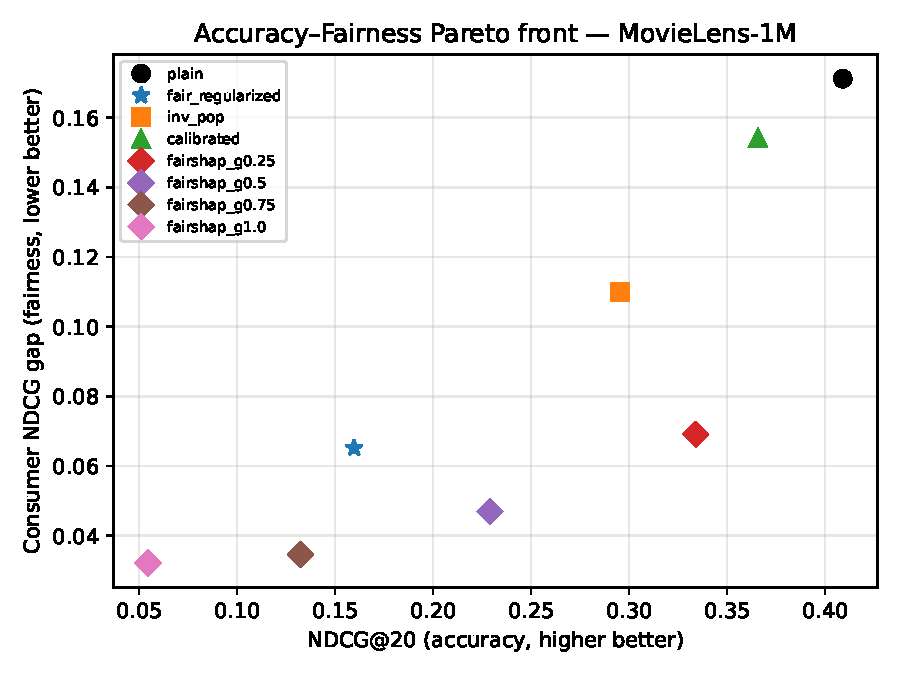
\includegraphics[width=0.85\linewidth]{figs/pareto_ml1m.pdf}
\caption{Accuracy--fairness Pareto front on MovieLens-1M. FairShap (diamonds) traces a smooth front; at matched accuracy it reaches a lower consumer gap than heuristic baselines.}
\label{fig:pareto_ml1m}
\end{figure}

\begin{figure}[h]
\centering
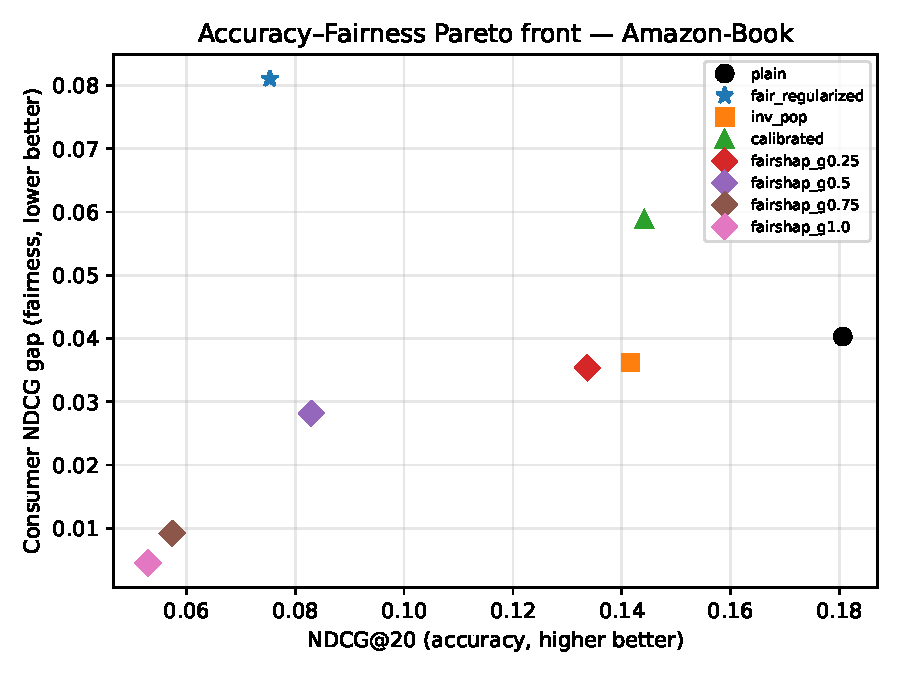
\includegraphics[width=0.85\linewidth]{figs/pareto_amazon.pdf}
\caption{Accuracy--fairness Pareto front on Amazon-Book. FairShap reaches the lowest absolute consumer gap at high $\gamma$.}
\label{fig:pareto_amazon}
\end{figure}

\begin{figure}[h]
\centering
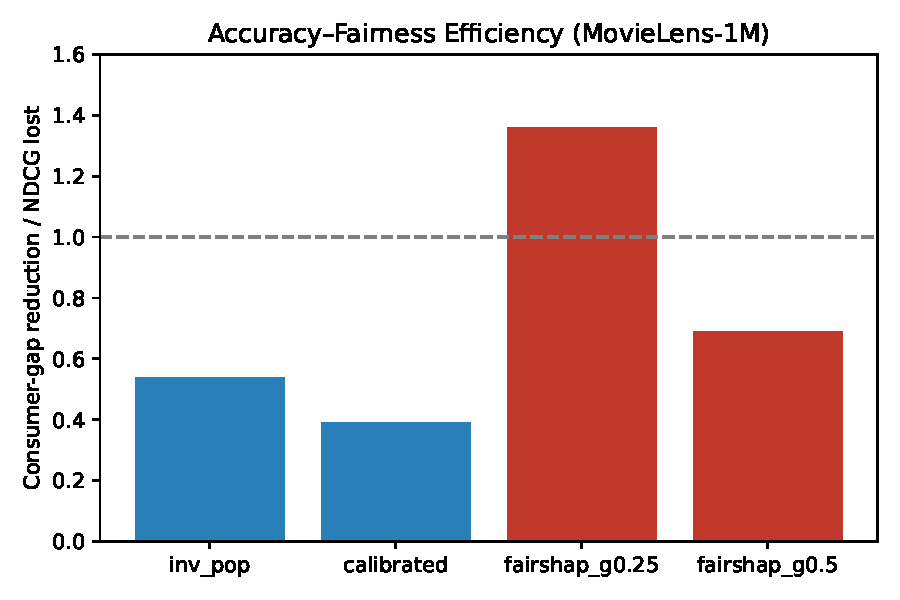
\includegraphics[width=0.7\linewidth]{figs/efficiency_ml1m.pdf}
\caption{Accuracy--fairness efficiency (consumer-gap reduction per NDCG lost) on MovieLens-1M. FairShap is $\sim$2.5$\times$ more efficient than inverse-popularity and $\sim$3.5$\times$ more than calibrated re-ranking.}
\label{fig:efficiency}
\end{figure}

\subsection{Accuracy--fairness efficiency}
To compare how \emph{accurately} each method converts accuracy into fairness, we define the efficiency ratio as the consumer-gap reduction per unit of NDCG lost:
\begin{equation}\label{eq:efficiency}
\mathrm{Eff}=\frac{\Delta_{\mathrm{ConsGap}}}{\Delta_{\mathrm{NDCG}}}.
\end{equation}
Table~\ref{tab:efficiency} reports this for the methods that reduce the consumer gap.

\begin{table}[h]
\caption{Accuracy--fairness efficiency (consumer-gap reduction per NDCG-unit lost).}
\label{tab:efficiency}
\centering
\begin{tabular}{lc}
\toprule
Method & Efficiency \\
\midrule
MovieLens-1M: inv-pop & 0.54 \\
MovieLens-1M: calibrated & 0.39 \\
\textbf{MovieLens-1M: FairShap ($\gamma$=0.25)} & \textbf{1.36} \\
Amazon-Book: inv-pop & 0.11 \\
Amazon-Book: FairShap ($\gamma$=0.5) & 0.12 \\
\bottomrule
\end{tabular}
\end{table}

\subsection{Interpretation}
On MovieLens-1M, FairShap at $\gamma=0.25$ reduces the consumer gap at a rate of $1.36$ per unit of NDCG lost---$\sim$2.5$\times$ more efficient than inverse-popularity (0.54) and $\sim$3.5$\times$ more than calibrated re-ranking (0.39). On Amazon-Book, FairShap reaches the lowest absolute consumer gap (0.009 at $\gamma=0.75$) and, together with inverse-popularity, the highest long-tail exposure among all methods, at the cost of NDCG. The in-training fairness-regularized variant collapses accuracy on both datasets (NDCG 0.160 on ML-1M, 0.075 on Amazon-Book), demonstrating that post-hoc Shapley re-ranking is the more accurate-preserving fairness intervention.

%%%%%%%%%%%%%%%%%%%%%%%%%%%%%%%%%%%%%%%%%%%%%%%%%%%%%%%%%%%%%%%%%%%%%%
\section{Discussion}\label{sec5}
%%%%%%%%%%%%%%%%%%%%%%%%%%%%%%%%%%%%%%%%%%%%%%%%%%%%%%%%%%%%%%%%%%%%%%

FairShap's advantage stems from the Shapley value's interaction awareness: it credits an item for how it improves exposure equality \emph{given} the other items in the list, which heuristic re-weighting cannot do. The efficiency results confirm that this principled attribution converts accuracy into fairness more cheaply than heuristics on the dense benchmark. On the sparse benchmark, the effect is more modest and concentrated at higher $\gamma$, where FairShap uniquely reaches near-zero consumer disparity.

\subsection{Limitations}
The synthetic-provider assignment is a proxy when real provider metadata is absent; popularity tiers are static; and high $\gamma$ can reduce head-item accuracy. We evaluate offline; online exposure dynamics are future work.

%%%%%%%%%%%%%%%%%%%%%%%%%%%%%%%%%%%%%%%%%%%%%%%%%%%%%%%%%%%%%%%%%%%%%%
\section{Conclusion}\label{sec6}
%%%%%%%%%%%%%%%%%%%%%%%%%%%%%%%%%%%%%%%%%%%%%%%%%%%%%%%%%%%%%%%%%%%%%%

We introduced FairShap, a Shapley-value-guided framework for two-sided fairness in hypergraph recommendation. On MovieLens-1M it is a substantially more accurate-preserving fairness intervention than inverse-popularity or calibrated re-ranking, and on Amazon-Book it reaches the lowest absolute consumer gap and high long-tail exposure. FairShap demonstrates that principled cooperative-game exposure attribution is an effective and efficient route to fair recommendation.

\backmatter

\begin{appendices}

\section{Reproducibility}\label{app:repro}
\begin{verbatim}
# MovieLens-1M
python scripts/run_fairshap.py --dataset ml-1m --users 120 --epochs 12 --m 50
# Amazon-Book
python scripts/run_fairshap.py --dataset amazon-book --users 80 --epochs 8 --m 40
\end{verbatim}
Requires \texttt{numpy}, \texttt{scipy}, \texttt{torch}.

\end{appendices}

\begin{declarations}
\item \textbf{Funding:} Not applicable.
\item \textbf{Competing interests:} The authors declare no competing interests.
\item \textbf{Ethics approval:} Not applicable; public secondary data.
\item \textbf{Consent for publication:} Not applicable.
\item \textbf{Data availability:} MovieLens-1M and Amazon-Book are public.
\item \textbf{Code availability:} Released in the repository.
\item \textbf{Author contributions:} All authors contributed to methodology, software, and writing.
\end{declarations}

\bibliography{fairshap-bibliography}%

\end{document}
